\section{Window-tolerant F1 (W-F1)}
\label{app:wf1}

This appendix provides the formal mathematical definition of the
window-tolerant F1 metric used throughout the paper. The main text
remains fully interpretable without consulting this appendix.

Let a dialogue $d$ consist of $T_d$ turns, with gold boundary indices
$G_d \subset \{1,\dots,T_d-1\}$ and predicted boundary indices
$P_d \subset \{1,\dots,T_d-1\}$. Let $w \ge 0$ denote the tolerance window.

\myparagraph{Window-coverage matching}
Define the number of window-matched predicted boundaries
\[
\mathrm{TP}_d
= \left|\left\{
p \in P_d \;:\; \exists g \in G_d \text{ such that } |p-g| \le w
\right\}\right|,
\]
and the number of recovered gold boundaries
\[
\mathrm{MG}_d
= \left|\left\{
g \in G_d \;:\; \exists p \in P_d \text{ such that } |p-g| \le w
\right\}\right|.
\]
Under this window-coverage convention, multiple predicted boundaries may be
matched to the same gold boundary, while each gold boundary contributes at most
once to recall.

\myparagraph{Dialogue-level precision and recall}
Precision and recall are defined per dialogue with explicit empty-set handling:
\[
\mathrm{Prec}_d =
\begin{cases}
\mathrm{TP}_d / |P_d|, & |P_d| > 0, \\
1, & |P_d| = 0 \wedge |G_d| = 0, \\
0, & |P_d| = 0 \wedge |G_d| > 0,
\end{cases}
\]
\[
\mathrm{Rec}_d =
\begin{cases}
\mathrm{MG}_d / |G_d|, & |G_d| > 0, \\
1, & |G_d| = 0 \wedge |P_d| = 0, \\
0, & |G_d| = 0 \wedge |P_d| > 0.
\end{cases}
\]

\myparagraph{Dialogue-level W-F1}
The window-tolerant F1 score for dialogue $d$ is
\[
\mathrm{W\text{-}F1}_d =
\begin{cases}
\displaystyle
\frac{2\,\mathrm{Prec}_d\,\mathrm{Rec}_d}
     {\mathrm{Prec}_d + \mathrm{Rec}_d},
& \mathrm{Prec}_d + \mathrm{Rec}_d > 0, \\
0, & \text{otherwise}.
\end{cases}
\]

\myparagraph{Dataset-level aggregation}
Dataset-level W-F1 is computed as a macro average over dialogues:
\[
\mathrm{W\text{-}F1}
= \frac{1}{|D|} \sum_{d \in D} \mathrm{W\text{-}F1}_d .
\]

\myparagraph{Scope note}
This definition specifies the W-F1 variant used throughout this paper and should
not be assumed equivalent to other window-tolerant F1 formulations that employ
different matching or aggregation rules.

\myparagraph{Alternative (not used): one-to-one window matching}
For completeness, we define a one-to-one variant that credits at most one prediction
per gold boundary. Let $H_d$ be a bipartite graph with left nodes $P_d$, right nodes $G_d$,
and an edge $(p,g)$ iff $|p-g|\le w$. Let $M_d$ be a maximum-cardinality matching in $H_d$,
and define $TP^{1{:}1}_d \coloneqq |M_d|$. Then
\[
\mathrm{Prec}^{1{:}1}_d = \frac{TP^{1{:}1}_d}{|P_d|},\qquad
\mathrm{Rec}^{1{:}1}_d = \frac{TP^{1{:}1}_d}{|G_d|},
\]
with the same empty-set conventions as above, and
$\mathrm{W\text{-}F1}^{1{:}1}_d$ as the harmonic mean of
$\mathrm{Prec}^{1{:}1}_d$ and $\mathrm{Rec}^{1{:}1}_d$.
All results in this paper use the window-coverage definition presented here
(i.e., $TP_d$ and $MG_d$ as defined above), not the one-to-one variant.

\section{Purity and Coverage}
\label{app:purity-coverage}
This appendix defines the purity and coverage diagnostics used to
characterize gold-relative segment alignment in
Section~\ref{sec:evaluation-metrics}.

Let a dialogue $d$ be segmented into predicted segments
$P^{\mathrm{seg}}_d = \{p_1,\dots,p_m\}$ and gold segments
$G^{\mathrm{seg}}_d = \{g_1,\dots,g_n\}$, where each segment is a contiguous span
of turns and the segmentations form partitions of $\{1,\dots,T_d\}$.

For a segment $s = [a,b]$, let $|s| = b-a+1$ denote its length in turns, and for
two segments $s$ and $t$ define their overlap
\[
|s \cap t| = \max\!\left(0,\; \min(b_s,b_t) - \max(a_s,a_t) + 1\right).
\]

\myparagraph{Segment-level purity and coverage}
For a predicted segment $p \in P^{\mathrm{seg}}_d$, define its purity as
\[
\mathrm{Purity}(p)
= \max_{g \in G^{\mathrm{seg}}_d} \frac{|p \cap g|}{|p|}.
\]
For a gold segment $g \in G^{\mathrm{seg}}_d$, define its coverage as
\[
\mathrm{Coverage}(g)
= \max_{p \in P^{\mathrm{seg}}_d} \frac{|p \cap g|}{|g|}.
\]

\myparagraph{Dialogue-level segment averages}
Segment-averaged purity and coverage for dialogue $d$ are
\[
\mathrm{Purity}_d
= \frac{1}{|P^{\mathrm{seg}}_d|}\sum_{p \in P^{\mathrm{seg}}_d}
\mathrm{Purity}(p)
= \frac{1}{|P^{\mathrm{seg}}_d|}\sum_{p \in P^{\mathrm{seg}}_d}
\max_{g \in G^{\mathrm{seg}}_d} \frac{|p \cap g|}{|p|},
\]
\[
\mathrm{Coverage}_d
= \frac{1}{|G^{\mathrm{seg}}_d|}\sum_{g \in G^{\mathrm{seg}}_d}
\mathrm{Coverage}(g)
= \frac{1}{|G^{\mathrm{seg}}_d|}\sum_{g \in G^{\mathrm{seg}}_d}
\max_{p \in P^{\mathrm{seg}}_d} \frac{|p \cap g|}{|g|}.
\]
This formulation weights each segment equally regardless of length.

\myparagraph{Dataset-level aggregation}
Dataset-level purity and coverage are computed as macro averages over dialogues:
\[
\mathrm{Purity}
= \frac{1}{|D|} \sum_{d \in D} \mathrm{Purity}_d,
\qquad
\mathrm{Coverage}
= \frac{1}{|D|} \sum_{d \in D} \mathrm{Coverage}_d.
\]

\section{Monotonicity Properties}
\label{app:monotonicity}
This appendix discusses monotonicity properties of purity and coverage
under segment refinement.

\myparagraph{Segment-averaged purity (as used in this paper)}
The segment-averaged purity defined in Appendix~B is \emph{not} monotone
under refinement. Splitting a low-purity segment into subsegments
(each with purity at least as high) increases the number of segments in
the average, which can decrease overall dialogue-level purity if the
split segment had below-average purity. This property is acceptable for
our diagnostic purposes: purity is used to detect cross-gold mixing,
not as an optimization target.

\myparagraph{Alternative: turn-weighted purity (not used)}
A turn-weighted variant, $\mathrm{Purity}^{\mathrm{micro}}_d = (1/T_d)\sum_p \max_g |p \cap g|$,
\emph{is} monotone under refinement: splitting segment $p$ into $p_1,\dots,p_k$
yields $\sum_i \max_g |p_i \cap g| \ge \max_g |p \cap g|$ since each
subsegment's best-matching gold overlap is at least its overlap with $p$'s
best-matching gold. However, turn-weighted purity over-credits long segments,
which is why we use segment-averaged purity.

\myparagraph{Coverage under refinement}
Coverage is anti-monotone under refinement: splitting predicted segments
cannot increase the maximum overlap between any gold segment and a single
predicted segment. This holds for both segment-averaged and turn-weighted
variants.

\section{Boundary canonicalization}
\makeatletter
\def\@currentlabelname{Window-tolerant F1 (W-F1)}
\makeatother
\label{app:canonicalization}

All datasets are converted to a canonical message sequence $m_1,\dots,m_T$ per dialogue, where each $m_t$ corresponds
to one dataset-provided utterance after filtering (below). Candidate boundary indices are the between-message positions
$i\in\{1,\dots,T-1\}$.

\myparagraph{Filtering}                                                                 
We (i) retain all dialogue turns from both speakers (user and agent/assistant), removing only dataset-level metadata headers where present (e.g., meeting       
preambles in QMSum), (ii) preserve speaker role labels but do not include them in utterance text, and (iii) remove empty or whitespace-only utterances if any   
exist. After filtering, messages are reindexed so that all boundary indices refer to positions in the filtered sequence.                                        

\myparagraph{Gold boundary extraction}
For each dataset, we define the gold boundary set $G_d\subseteq\{1,\dots,T_d-1\}$ using the dataset's native segment
annotation as follows:
\begin{itemize}
\item \textbf{Datasets with segment IDs per utterance:} let $\ell_t$ be the segment ID for message $m_t$; then
  $G_d = \{\, i : \ell_i \ne \ell_{i+1}\,\}$.
\item \textbf{Datasets with explicit boundary markers:} let $b_t\in\{0,1\}$ indicate that $m_t$ starts a new segment;
  then $G_d = \{\, i : b_{i+1}=1\,\}$.
\item \textbf{Domain-/state-labeled datasets:} let $\texttt{label}_t$ denote the dataset-provided label for message $m_t$; then
  $G_d=\{\, i : \texttt{label}_i \ne \texttt{label}_{i+1}\,\}$.
\end{itemize}

\myparagraph{Dataset-specific notes}
Table~\ref{tab:canon} summarizes the canonicalization rules; complete
extraction implementations are in the accompanying code repository.

{\hyphenpenalty=10000
\exhyphenpenalty=10000

\begin{table}[t]
\centering
\small
\setlength{\tabcolsep}{6pt}
\begin{tabularx}{\linewidth}{
l
c
>{\raggedright\arraybackslash}X
>{\raggedright\arraybackslash}X
}
\toprule
Dataset &
Unit &
Annotation $\rightarrow G_d$ rule &
Filtering notes \\
\midrule
DialSeg711 & U &
Segment ID change between consecutive utterances &
All turns retained; indexed consecutively \\

SuperSeg & U &
Segment ID change between consecutive utterances &
All turns retained; indexed consecutively \\

TIAGE & U &
Task/topic segment change between consecutive utterances &
All turns retained; indexed consecutively \\

MultiWOZ & U &
Domain label change between consecutive utterances &
All turns retained; indexed consecutively \\

DailyDialog & U &
Topic category change between consecutive utterances &
All turns retained; indexed consecutively \\

Taskmaster & U &
Task or subtask label change between consecutive utterances &
All turns retained; indexed consecutively \\

Topical-Chat & U &
Conversation topic change between consecutive utterances &
All turns retained; indexed consecutively \\

QMSum & T &
Section/topic boundary between adjacent speaker turns &
Meeting metadata removed \\
\bottomrule
\end{tabularx}
\caption{Boundary canonicalization details required to reproduce gold
boundary sets $G_d$ from each dataset.
Unit codes: \textbf{U} = each message is a boundary candidate (typical for two-party dialogues where speakers alternate);
\textbf{T} = boundaries occur only at speaker changes, grouping consecutive sentences from the same speaker into one unit (used for multi-party meeting transcripts like QMSum).}
\label{tab:canon}
\end{table}
}

\section{Full Stage~3 Calibrated Results Across All Datasets}
\label{app:stage3}

All results reported in this appendix use the identical Stage~3 evaluation pipeline
and are computed exclusively on \emph{test splits}:
a single model checkpoint after Stage~2 training,
a single global temperature calibrated on the SuperSeg validation split,
fixed boundary canonicalization,
and fixed boundary-selection parameters.
No information from any test split is used during training or calibration.
The evaluation protocol follows the train/validation/test split specification
summarized in Table~\ref{tab:training-protocol}.

The main text (Section~\ref{sec:stage3}) reports Stage~3 calibrated results on three
representative datasets spanning sparse, medium, and dense annotation
regimes. To substantiate the cross-dataset claims made in Sections~4 and~7,
this appendix reports the same Stage~3 evaluation
metrics for all eight datasets used in this study: DialSeg711,
SuperSeg, TIAGE, MultiWOZ, DailyDialog, Taskmaster,
Topical-Chat, and QMSum.

All results in Table~\ref{tab:stage3-all8} were computed using the
identical Stage~3 evaluation pipeline as the main Stage~3 results
(Table~\ref{tab:stage3}): a single globally calibrated temperature
($T=0.976$), identical boundary canonicalization, fixed boundary
selection parameters, and the evaluation definitions in Section~\ref{sec:evaluation-metrics}.

We report window-tolerant boundary detection (W-F1 with a $\pm 1$
message tolerance), boundary density relative to gold annotations
(BOR), and segment coherence diagnostics (purity and coverage), along
with predicted and gold boundary counts. Strict exact-match boundary
F1 is omitted here because it is highly sensitive to aggregation
choice (e.g., micro vs.\ macro averaging) and boundary sparsity, and
it is not a primary diagnostic in the proposed evaluation objective.

\begin{table}[t]
  \centering
  \small
  \begin{tabular}{lcccccc}
    \toprule
    Dataset & W-F1 & BOR & Purity & Coverage & Pred./Gold \\
    \midrule
    DialSeg711    & 0.708 & 1.38  & 0.875 & 0.772 & 2820/2042 \\
    SuperSeg      & 0.520 & 0.50  & 0.765 & 0.938 & 1461/2923 \\
    TIAGE         & 0.474 & 0.52  & 0.741 & 0.913 & 107/207   \\
    DailyDialog   & 0.383 & 0.62  & 0.753 & 0.911 & 125/200   \\
    MultiWOZ      & 0.694 & 1.29  & 0.901 & 0.833 & 1437/1117 \\
    Taskmaster    & 0.278 & 3.10  & 0.926 & 0.594 & 607/196   \\
    Topical-Chat  & 0.290 & 2.77  & 0.922 & 0.641 & 543/196   \\
    QMSum         & 0.151 & 10.40 & 0.962 & 0.474 & 2195/211  \\
    \bottomrule
  \end{tabular}
  \caption{\textbf{Stage~3 calibrated results for all eight datasets.}
    Metrics computed under the same calibrated Stage~3 pipeline used in Table~\ref{tab:stage3},
    with identical model checkpoint, temperature calibration ($T=0.976$), boundary canonicalization,
    and selection settings.
    This appendix reports a subset of diagnostics focused on boundary density and segment coherence;
    strict exact-match F1 is intentionally omitted because it is highly sensitive to aggregation and
    boundary sparsity and is not a primary diagnostic in the proposed evaluation objective.}
  \label{tab:stage3-all8}
\end{table}

\section{Adaptive Boundary Selection}
\label{app:adaptive}

This appendix provides a formal specification of the adaptive boundary
selection mechanism referenced in Section~\ref{sec:boundary-selection}.

\myparagraph{Definitions and target rate}
Candidate boundaries correspond to between-message indices
$i \in \{1,\ldots,T{-}1\}$, where $i$ denotes the position between messages
$(m_i, m_{i+1})$.

Let $C(t)$ denote the number of candidate positions processed up to time $t$, and
let $S(t)$ denote the number of boundaries committed up to time $t$. The adaptive
controller targets a boundary \emph{selection rate}
\[
\rho \;=\; \mathbb{E}\!\left[\frac{S(t)}{C(t)}\right],
\]
measured per processed candidate position (not per message or per dialogue).

\myparagraph{Evidence accumulation}
Each candidate position $i$ maintains an accumulated evidence value $e_i(t)$.
When a candidate $i$ first becomes available, a boundary score $s_i$ is computed
once using frozen reference windows anchored at that time. This score remains
fixed thereafter.

As additional post-boundary context becomes available, evidence is accumulated
according to
\[
e_i(t{+}1) \;=\; e_i(t) + s_i .
\]
This implements a time-to-threshold integrator: candidates with higher initial
scores $s_i$ reach the commitment threshold faster than candidates with lower
scores. Freezing the score at the time of first availability ensures that the
commitment decision reflects the strength of the boundary signal at the point of
topic departure, rather than being confounded by subsequent context that may
diverge further or return to the original topic. The adaptive threshold
$\tau(t)$ (below) provides the primary density control mechanism.

\myparagraph{Boundary commitment rule}
At time $t$, a candidate boundary at position $i$ is committed if and only if
\[
e_i(t) \ge \tau(t)
\quad\text{and}\quad
|i - b| \ge g \;\;\forall b \in \mathcal{B},
\]
where $\tau(t)$ is the current decision threshold, $g$ is a minimum spacing
constraint, and $\mathcal{B}$ is the set of previously committed boundaries.
Candidates violating the spacing constraint are suppressed.

\myparagraph{Adaptive threshold controller}
The threshold $\tau(t)$ is updated online to enforce the target selection rate
$\rho$. Let $\hat{\rho}(t)$ denote the empirical selection rate over the most
recent $W$ processed candidates (or all candidates if fewer than $W$ have been
seen). The controller update is
\[
\tau(t{+}1) \leftarrow \tau(t) + \eta\,(\hat{\rho}(t) - \rho),
\]
where $\eta > 0$ is a step size. Increasing $\tau$ reduces boundary commits, while
decreasing $\tau$ increases them.

\myparagraph{Pseudocode}
The following pseudocode provides a complete operational realization of the
adaptive boundary selection procedure described above.

\begin{algorithm}[t]
\caption{Adaptive boundary selection}
\label{alg:adaptive}

\KwIn{target rate $\rho$, spacing $g$, window size $W$, step size $\eta$,
initial threshold $\tau(0)$}
\KwOut{committed boundary set $\mathcal{B}$}

$\mathcal{B} \leftarrow \emptyset$\;
Initialize counters $C \leftarrow 0$, $S \leftarrow 0$\;

\For{each time step $t$ as messages arrive}{
  \For{each newly available candidate $i$}{
    compute frozen score $s_i$; set $e_i \leftarrow 0$\;
  }
  \For{each active candidate $i$}{
    $e_i \leftarrow e_i + s_i$\;
    $C \leftarrow C + 1$\;
    \If{$e_i \ge \tau(t)$ \textbf{and} $|i-b| \ge g$ for all $b \in \mathcal{B}$}{
      $\mathcal{B} \leftarrow \mathcal{B} \cup \{i\}$\;
      $S \leftarrow S + 1$\;
    }
  }
  compute $\hat{\rho}(t)$ over last $W$ candidates\;
  $\tau(t{+}1) \leftarrow \tau(t) + \eta(\hat{\rho}(t)-\rho)$\;
}
\end{algorithm}

\myparagraph{Remarks}
The adaptive controller operates on candidate positions rather than messages,
making the target rate invariant to dialogue length. Freezing the boundary score
avoids repeatedly re-scoring shifting contexts, and ensures that high-scoring
candidates are committed before low-scoring ones under time pressure imposed by
the adaptive threshold. When $\tau(t)$ is held fixed and accumulation is
disabled, the procedure reduces to the static selection rule used in the main
experiments.

\FloatBarrier

\section{Robustness to Matching Convention}
\label{app:wf1:matching}

This appendix verifies that the density confound identified in the main paper is not an artifact of the many-to-one window-coverage matching used for W-F1. We evaluate two additional matching conventions: one-to-one tolerant matching and strict exact-position matching.

\myparagraph{One-to-one tolerant matching}
Let $P$ be predicted boundaries and $G$ gold boundaries, and let $w$ be the tolerance window.
Construct a bipartite graph with edges $(p,g)$ when $|p-g|\le w$.
Compute a maximum-cardinality matching $M \subseteq P \times G$ (ties broken arbitrarily or by minimum total distance).
Define $\mathrm{TP}=|M|$, $\mathrm{FP}=|P|-\mathrm{TP}$, and $\mathrm{FN}=|G|-\mathrm{TP}$, and compute precision/recall/F1 in the usual way.
This enforces the one-to-one constraint that each predicted (resp.\ gold) boundary can be credited at most once.

\myparagraph{Exact F1 (strict position matching)}
Exact F1 requires predicted boundaries to match gold boundary positions exactly, with no tolerance window ($w=0$). This is the strictest evaluation and reflects what most published dialogue segmentation work reports.

\myparagraph{Results}
Figure~\ref{fig:matching_comparison} shows density--quality curves under all three matching conventions. The strong positive correlation between boundary density (BOR) and F1-based metrics persists across all matching semantics. Table~\ref{tab:matching_correlations} quantifies this for the neural scorer.

Notably, the exact F1 curves exhibit flatter peaks and sharper decline under oversegmentation compared to tolerant variants. Under strict matching, boundaries cannot be ``close enough'' to count---excess boundaries are penalized directly. Nevertheless, the correlation remains strong ($r > 0.83$) up to the peak, demonstrating that the confound is fundamental to F1-based evaluation under sparse boundary labels, not an artifact of tolerant matching protocols.

\begin{table}[t]
  \centering
  \small
  \begin{tabular}{llcc}
    \toprule
    Dataset & Metric & $r$ & Optimal BOR \\
    \midrule
    DialSeg711 & W-F1 (many-to-one) & 0.88 & 1.67 \\
    DialSeg711 & W-F1 (one-to-one) & 0.86 & 1.60 \\
    DialSeg711 & Exact F1 & 0.87 & 1.54 \\
    \midrule
    SuperSeg & W-F1 (many-to-one) & 0.88 & 0.95 \\
    SuperSeg & W-F1 (one-to-one) & 0.91 & 1.01 \\
    SuperSeg & Exact F1 & 0.83 & 0.88 \\
    \bottomrule
  \end{tabular}
  \caption{Pearson correlation between BOR and F1 metrics for the neural scorer. Strong positive correlations persist across all matching conventions. Optimal BOR shifts slightly lower under stricter matching, but remains above 1.0 for DialSeg711.}
  \label{tab:matching_correlations}
\end{table}

\begin{figure}[ht]
  \centering
  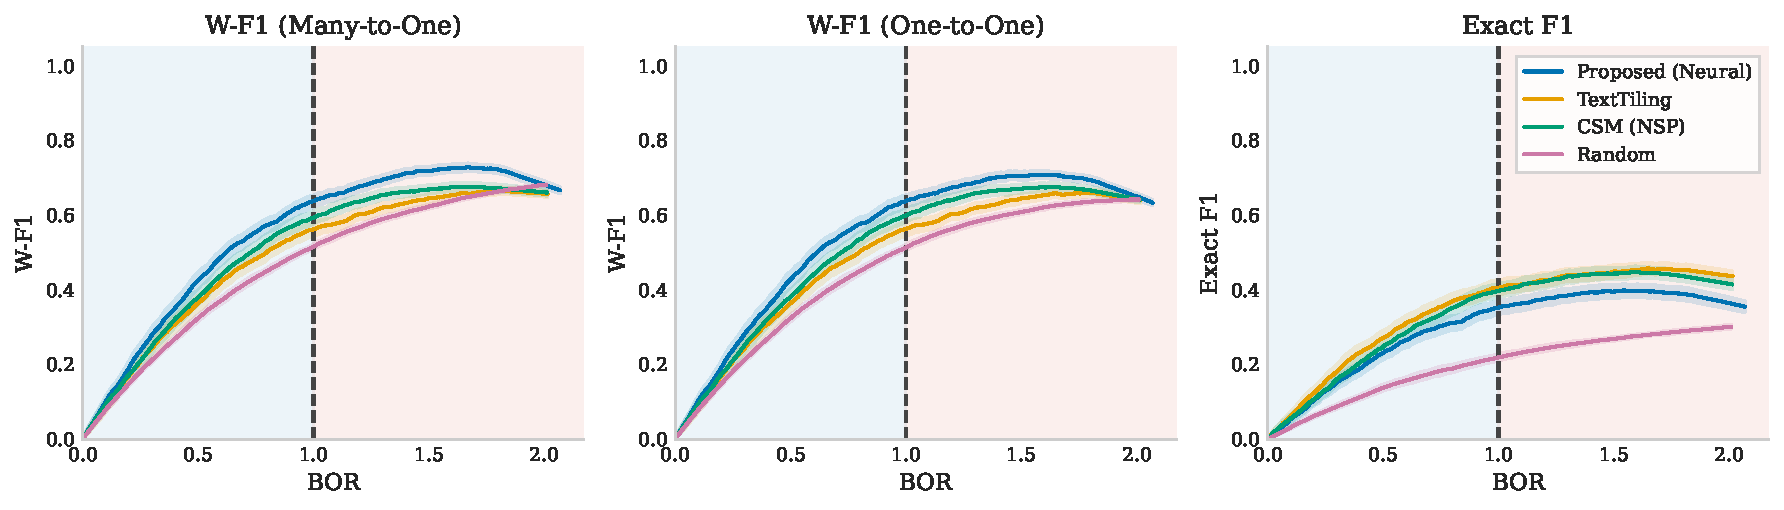
\includegraphics[width=\linewidth]{figures/appendix_g_dialseg711_v2.pdf}\\
\vspace{-12pt}
\noindent\makebox[\linewidth][c]{%
  \leaders\hbox{\rule{6pt}{0.3pt}\hspace{4pt}}\hskip0.9\linewidth
}
\vspace{4pt}
  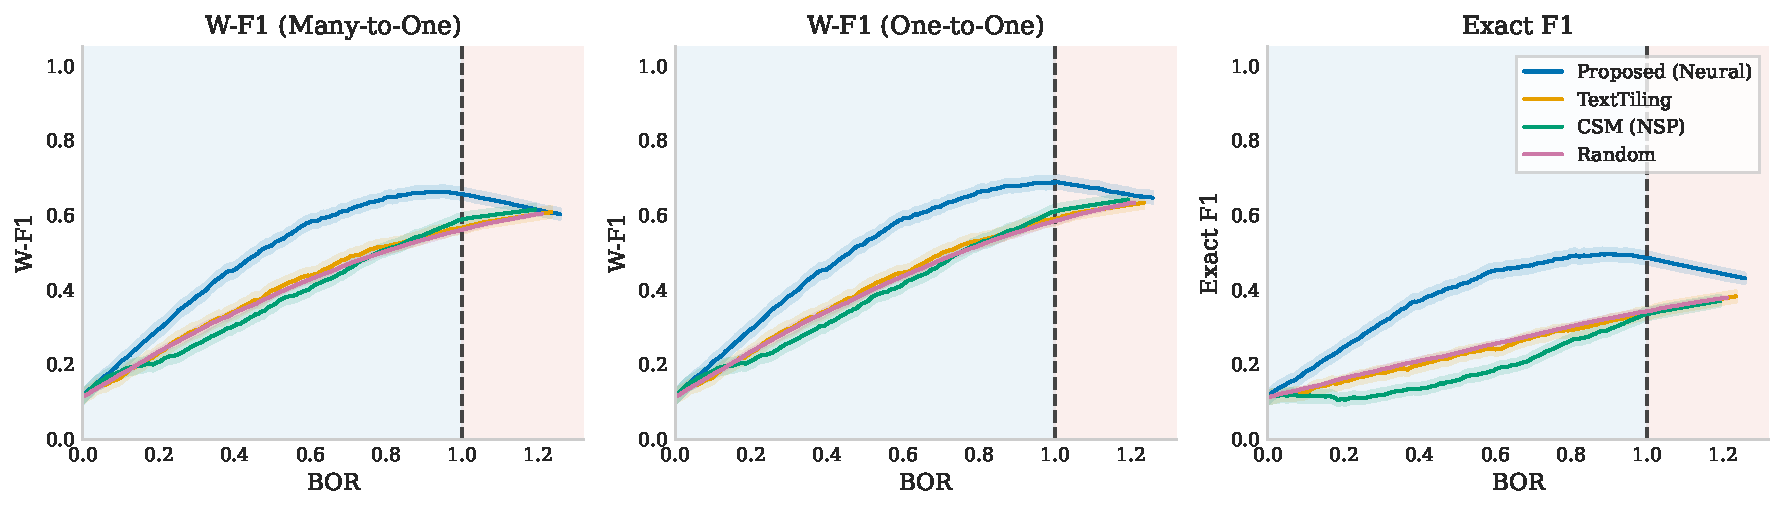
\includegraphics[width=\linewidth]{figures/appendix_g_superseg_v2.pdf}
  \caption{\textbf{Robustness of density--quality curves to matching convention.}
  Left: many-to-one (window-coverage) W-F1 used in the main paper.
  Center: one-to-one tolerant matching via maximum bipartite matching.
  Right: exact F1 with strict position matching ($w=0$).
  Shading indicates BOR $< 1$ (left of dashed line) and BOR $> 1$ (right).
  Across all three conventions, varying boundary density produces larger changes in F1 than switching between methods at matched density. Shaded regions indicate 95\% bootstrap confidence intervals.}
  \label{fig:matching_comparison}
\end{figure}

\section{Audit protocol and canonicalization details}
\label{app:audit}
\myparagraph{Controlled}
We fix: (i) boundary indexing and mapping to turn positions, (ii) the
tolerance window $w$, (iii) metric implementations, and (iv) the
operating-point protocol used to select or sweep thresholds to induce a
range of BOR values for each method.

\myparagraph{Not controlled}
We do not attempt to replicate each method's original preprocessing,
training regime, or originally reported threshold tuning; therefore, we
do not interpret discrepancies with published single-number reports as
errors, and we do not attribute differences uniquely to modeling choices
independent of preprocessing.
\FloatBarrier
